\documentclass[nobib]{tufte-handout}

\usepackage[utf8]{inputenc}
\usepackage[autostyle=true,german=quotes]{csquotes}
\usepackage{hyphsubst} %\HyphSubstLet{ngerman}{ngerman-x-latest} % für die Trennung von zwei-schrittig
\usepackage[ngerman]{babel}   % neue deutsche Rechtschreibung (z. B. auch für Silbentrennung)
\usepackage[htt]{hyphenat}  % Umbruch bei \texttt

\title{Vorbereitung für das Seminar\\
\enquote{Maschinelles Lernen: Potentiale und Risiken}}

\author{Marvin Kastner \href{mailto:marvin.kastner@tuhh.de}{<marvin.kastner@tuhh.de>}}

%\date{28 March 2010} % without \date command, current date is supplied

\usepackage{graphicx} % allow embedded images
  \setkeys{Gin}{width=\linewidth,totalheight=\textheight,keepaspectratio}
  \graphicspath{{graphics/}} % set of paths to search for images

\usepackage{xurl}  % break url

\usepackage[
	type={CC},
	modifier={by},
	version={4.0},
	imagemodifier={-eu-88x31},
]{doclicense}


\begin{document}

\maketitle% this prints the handout title, author, and date

In dieser Anleitung werden die Schritte aufgezählt, die von den Seminarteilnehmenden selbständig \emph{vor} Beginn des Seminars auf dem eigenen Endgerät (Laptop, MacBook, ...) durchgeführt werden müssen.
Bitte planen Sie hierfür zirka eine Stunde ein, bei langsamen Internet oder weniger leistungsfähigen Endgeräten entsprechend mehr.
Falls Sie während des Seminars kein eigenes leistungsfähiges Endgerät (z.\,B.\ nur einen alten Laptop oder ein Tablet) zur Verfügung haben sollten, sprechen Sie bitte frühzeitig die Seminarleitung an.

Übrigens -- falls Sie Anaconda bereits installiert haben sollten, stellen Sie bitte sicher, dass Ihre Version aktuell ist.
Nachdem Sie conda ggf.\ geupdatet haben, können Sie direkt zum Abschnitt \emph{\nameref{sec:git-clone}} springen und die conda-Umgebung mit den benötigten Bibliotheken installieren.


\section{Installation von JupyterLab}

Gehen Sie auf
\url{https://www.anaconda.com/download} 
und laden Sie die Anaconda-Version für Ihr Betriebssystem herunter.
Anaconda ist eine Python-Distribution, die vorkompilierte Bibliotheken ausliefert und damit den Aufwand beim Installieren ebendieser minimiert.
Der Download-Bereich der Webseite sollte wie in Abbildung\,\ref{fig:anaconda-download-section} aussehen.

\begin{marginfigure}
  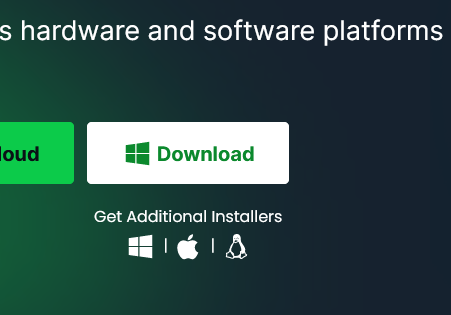
\includegraphics{anaconda_download_section}
  \caption{Der Download-Bereich von Anaconda (Ausschnitt).}%
\label{fig:anaconda-download-section}
\end{marginfigure}

Falls Sie auf Ihrem Endgerät mithilfe von zwei Accounts streng zwischen administrativen Tätigkeiten auf der einen Seite und dem alltäglichen Arbeiten mit stark eingeschränkten Rechten auf der anderen Seite unterscheiden, werden Sie vermutlich versuchen, Anaconda mit dem Administrator- bzw.\ root-Account zu installieren und danach mit dem anderen Account Anaconda zu nutzen.
Falls das auf Sie zutrifft, lesen Sie bitte die Notiz in der rechten Spalte.
\marginnote{%
Die Installation von Anaconda erfordert keine erhöhten Rechte.
Eine Installation mit einem Nutzer mit erhöhten Rechten kann u.\,U.\ dazu führen, dass Anaconda nur für diesen einen Nutzer mit erhöhten Rechten installiert ist bzw.\ dass es zu Problemen mit der Rechteverwaltung kommt.
In der Vergangenheit hat ein erneutes Installieren von Anaconda dieses Problem dann \emph{nicht} beheben können.
Lösungen für ein Setup mit mehreren Benutzern lassen sich unter
\url{https://docs.anaconda.com/anaconda/install/multi-user/}
finden.
}%
Wenn Sie sich, wie die meisten, nur mit einem Benutzer-Account arbeiten, sind Sie hiervon nicht betroffen.

Rufen Sie nach dem Download den Installer aus dem Download-Ordner auf und folgen Sie den Installationsschritten.
Konsultieren Sie im Fehlerfall offizielle Quellen des Anbieters
(wie z.\,B.\ \url{https://docs.anaconda.com/anaconda/install/})
oder Foren
(wie z.\,B.\ \url{https://stackoverflow.com}).


\newthought{Warum werden Jupyter Notebooks eingesetzt?}
Im Bereich Maschinelles Lernen und Data Science spielen Jupyter Notebooks eine  große Rolle.
Das Medienformat ist auf JSON-Basis und kann neben dem ausführbaren Code
u.\,a.\ auch
Text (d.\,h.\ Plaintext, Markdown, LaTeX und HTML),
Bilder,
Visualisierungen von Daten,
Videos und
Animationen
enthalten.
So können die Arbeitsschritte für Dritte nachvollziehbar in einem Dokument zentral dokumentiert und die Ergebnisse visualisiert werden.


\section{Bezug der Seminar-Materialien}
\label{sec:git-clone}

Klonen Sie das git-Repository
\url{https://github.com/1kastner/ml-potentials-and-risks},
damit Sie die Seminar-Materialien lokal haben -- dies umfasst nur den Programmierteil.
Am einfachsten ist es, wenn Sie die Dateien unterhalb des benutzer\-eigenen Ordners \texttt{Dokumente} ablegen
(unter Windows meist \texttt{C:\textbackslash{}Users\textbackslash{}BENUTZERNAME\textbackslash{}Documents}).
Denn dieser Ordner ist, wenn JupyterLab aus Anaconda heraus gestartet wird, direkt verfügbar.
Falls Sie noch nie mit git gearbeitet haben, lesen Sie bitte die nächsten Absätze.

\newthought{Warum sollte ich git lernen?}
Für die Versionsverwaltung ist git quasi der Standard und wird immer häufiger auch außerhalb der Software-Entwicklung eingesetzt.
Deswegen lohnt es sich für (fast) alle, sich Fähigkeiten mit diesem Tool anzueignen.
Es ist als ein Kommandozeilentool entwickelt worden, welches über
\url{https://git-scm.com/}
heruntergeladen werden kann.
Wer lieber grafische Oberflächen mag, kann sich einen der vielen GUI-Clients%
\sidenote{Eine Liste ist auf
\url{https://git-scm.com/download/gui/win}
zu finden.}
aussuchen.
Hier sollte neben dem Betriebssystem auch die ggf.\ kostenpflichtige Lizenz beachtet werden.
Einige Lizenzen unterscheiden z.\,B.\ zwischen der privaten Verwendung und der Verwendung im Arbeitskontext.
Bis zum Start des Seminars werden u.\,U.\ die Materialien noch überarbeitet oder erweitert.
Aktualisieren Sie also bitte regelmäßig Ihre vorliegende Version über ein \texttt{git pull} bzw.\ durch das Klicken auf den \enquote{Pull}-Button im GUI-Client Ihrer Wahl.

\newthought{Ist es für das Seminar zwingend notwendig, git zu lernen?}
Falls Ihnen git unbekannt ist und Sie keine Zeit dafür haben, sich mit git auseinanderzusetzen, gibt es auch die Möglichkeit, den Inhalt als ZIP-Ordner herunterzuladen.
Klicken Sie dafür auf den Button, wie er in Abbildung\,\ref{fig:github} zu sehen ist.
Falls Lernmaterialien später noch angepasst werden, müssen Sie diese dann allerdings erneut herunterladen und in einem neuen Ordner entpacken.

\begin{marginfigure}
  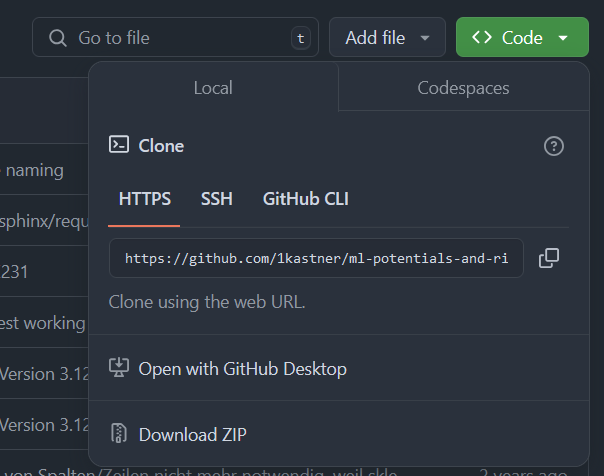
\includegraphics{github-zip}
  \caption{Ein GitHub-Repository bietet verschiedene Möglichkeiten zum Bezug der Inhalte an, auch den Download als ZIP-Datei.}%
\label{fig:github}
\end{marginfigure}


\section{Installation der Bibliotheken}

Mit der Installation von Anaconda ist u.\,a.\ die Applikation Anaconda Navigator ausgeliefert worden.
Mit dem Anaconda Navigator können die benötigten Bibliotheken automatisch installiert werden.
\marginnote{%
	Falls Sie Windows 10 verwenden und kein Multi-User-Setup haben, können Sie den folgenden Schritt dadurch abkürzen, dass Sie die Batch-Datei \texttt{create-env.bat} auf der Wurzelebene des Projekts durch einen Doppelklick ausführen.
	Im Falle einer Nachfrage bestätigen Sie, dass Sie dem Urheber der Batch-Datei vertrauen.
}
In der Abbildung\,\ref{fig:anaconda-navigator} sehen Sie unten den Button \enquote{Import}
(im Screenshot mit einer 1 markiert).
Klicken Sie diesen an.
Damit öffnet sich das Fenster \enquote{Import environment}.
Klicken Sie hier auf den Ordner in der Zeile, die mit 
\enquote{Local drive}
bezeichnet wird (mit einer 2 markiert).
Danach öffnet sich ein Fenster zur Datei-Auswahl
(mit einer 3 markiert),
in dem Sie dann zu den von GitHub bezogenen Dateien navigieren können.
Wählen Sie die Datei \texttt{environment.yml} aus
-- sie liegt auf der Wurzelebene des Projektordners --
und klicken Sie auf \enquote{Öffnen}.
Der zu erstellenden Umgebung können Sie nun einen sprechenden Namen geben, z.\,B.\ \texttt{ml-potentials-and-risks}.
Unter diesem Namen werden Sie die Umgebung später in Anaconda wiederfinden.
Das Erstellen der Umgebung beinhaltet den Download und die Installation der benötigten Bibliotheken; es nimmt für gewöhnlich mehrere Minuten in Anspruch.

\begin{figure}[h]
  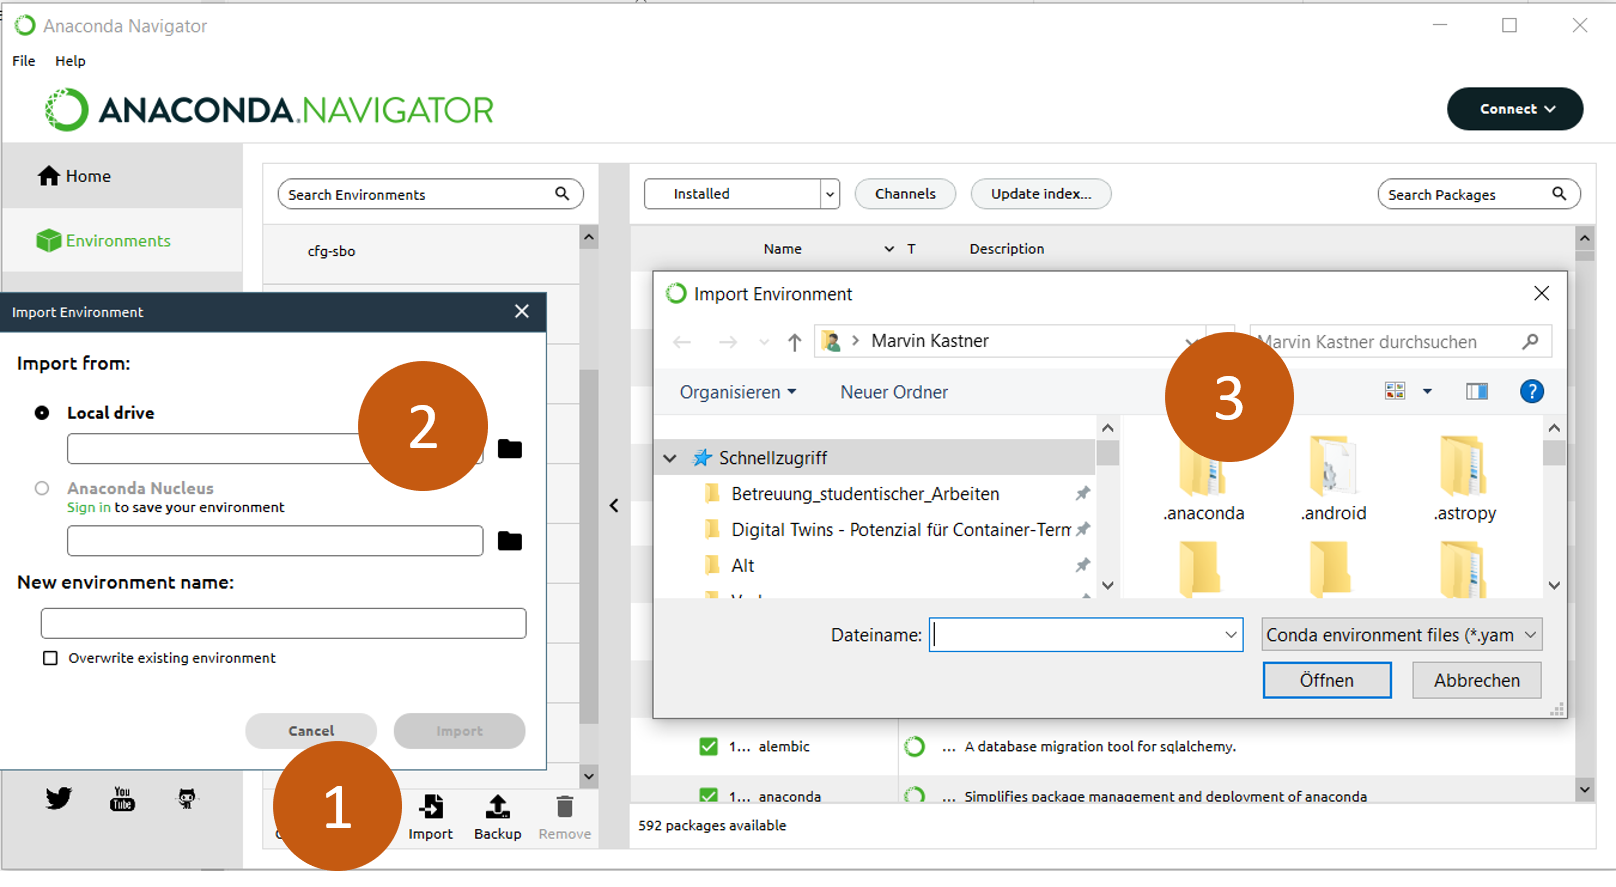
\includegraphics{anaconda-navigator-import-new-environment--mit-reihenfolge}
  \caption{Der Anaconda Navigator erlaubt das Importieren von \texttt{environment.yml}-Dateien.}%
\label{fig:anaconda-navigator}
\end{figure}

\newthought{Warum ist dieser Schritt notwendig?}
Die Jupyter Notebooks, die Sie soeben von GitHub bezogen haben, benötigen eine bestimmte Umgebung, damit sie wie gewünscht geöffnet und ausgeführt werden können.
Zu dieser Umgebung gehört z.\,B.\ ein Python-Interpreter mit einer bestimmten Python-Version ebenso wie eine Reihe ausgewählter Python-Bibliotheken.
Auf der obersten Ebene des git-Repositorys befindet sich die Datei \texttt{environment.yml}, in der alle Anforderungen an die Entwicklungsumgebung aufgeführt werden.
Die Struktur der Datei \texttt{environment.yml} ist von Anaconda vorgegeben und erlaubt es, die Abhängigkeiten von Bibliotheken automatisch aufzulösen.
Damit man auf einem Endgerät in verschiedenen Projekten unterschiedliche Versionen einer gleichen Bibliothek (und auch JupyterLab und andere Werkzeuge) haben kann,
strukturiert Anaconda die zu einem Projekt gehörenden Bibliotheken standardmäßig in Umgebungen (eng.\ Environments).
Für das Seminar erstellen wir die Umgebung
\texttt{ml-potentials-and-risks}
basierend auf der gegebenen \texttt{environment.yml}.

\newthought{Geht es denn nur über die GUI?}
Natürlich gibt es auch ein Kommandozeilentool, das mit Anaconda ausgeliefert worden ist.
Es heißt \texttt{conda}.
Unter Windows wird dieses Tool je nach Auswahl während der Installation nicht in die Pfad-Variable aufgenommen.
Es steht Ihnen aber auf jeden Fall in der
\emph{Anaconda Powershell Prompt} (basierend auf der PowerShell)
zur Verfügung.
Auf
\url{https://docs.conda.io/projects/conda/en/latest/user-guide/tasks/manage-environments.html#creating-an-environment-from-an-environment-yml-file}
wird erläutert, wie eine existierende \texttt{environment.yml} zur Erstellung einer Anaconda-Umgebung genutzt werden kann.

\section{Start von JupyterLab}

JupyterLab kann nun über den Anaconda Navigator gestartet werden.
In Abbildung~\ref{fig:start-jupyterlab} ist dies abgebildet.
\marginnote{%
	Falls Sie Windows 10 verwenden und kein Multi-User-Setup haben, können Sie den folgenden Schritt dadurch abkürzen, dass Sie die Batch-Datei
	\texttt{start-jupyterlab.bat}
	auf der Wurzelebene des Projekts durch einen Doppelklick ausführen.
	Dann ist auch die Wurzelebene des Projekts in JupyterLab der Wurzelordner.
}
Zunächst wird links im Menü
(im Screenshot mit einer 1 markiert)
\enquote{Home} ausgewählt.
Im zweiten Schritt muss die Umgebung
\texttt{ml-potentials-and-risks}
ausgewählt werden
(mit einer 2 markiert).
Danach startet ein Klick auf \texttt{Launch} die Anwendung JupyterLab im Browser
(mit einer 3 markiert).
Standardmäßig öffnet sich nun ein neuer Tab im Browser und JupyterLab zeigt zunächst den Inhalt vom Benutzer-Ordner an, wie in
Abbildung\,\ref{fig:inside-jupyterlab} zu sehen.
Von hier können Sie in den Unterordner \texttt{Dokumente} navigieren und zu den heruntergeladenen Seminarunterlagen gelangen.

\begin{figure}[h]
  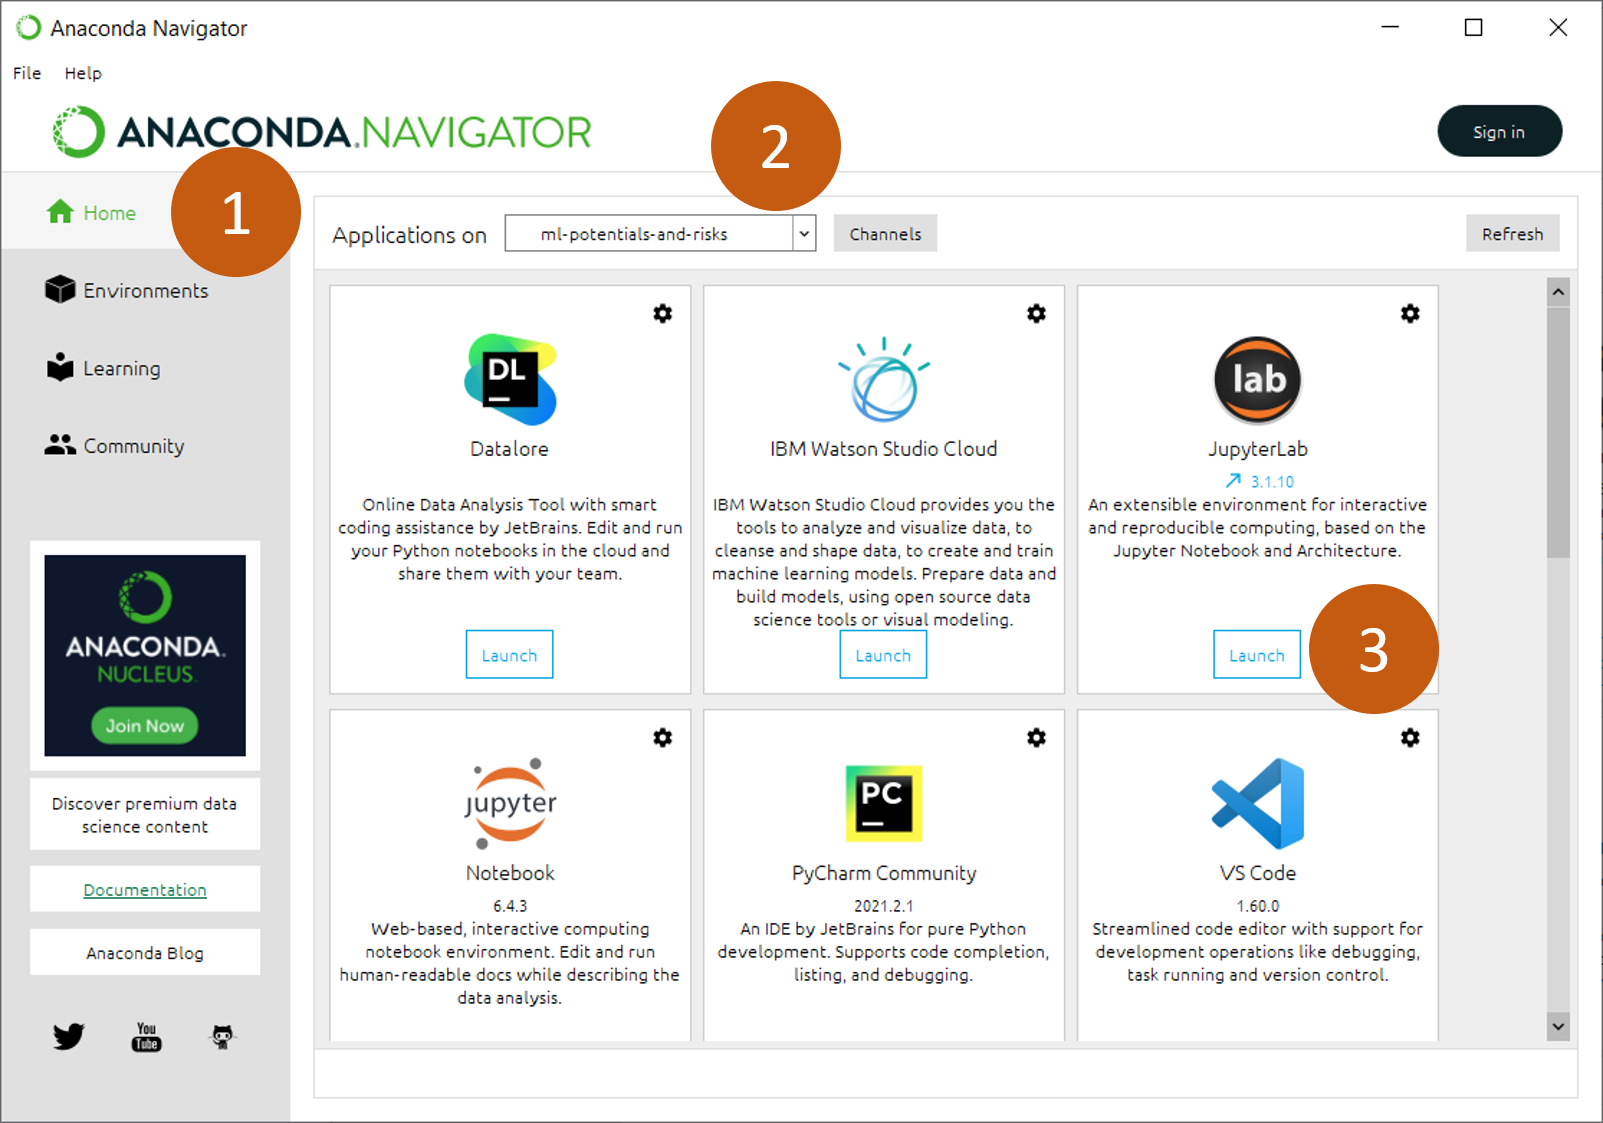
\includegraphics[trim={0 1.5cm 0 0},clip]{anaconda-navigator-jupyterlab--mit-reihenfolge}
  \caption{Aus dem Anaconda Navigator kann JupyterLab gleich in der richtigen Umgebung gestartet werden.%
  Die Reihenfolge und Sortierung der Logos kann variieren.}%
  \label{fig:start-jupyterlab}
\end{figure}

\begin{figure}[h]
  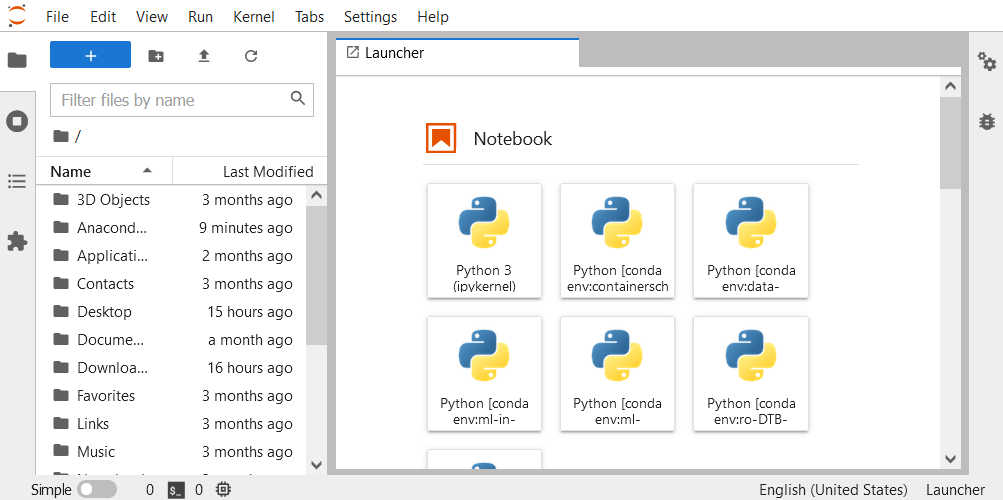
\includegraphics{jupyterlab-running}
  \caption{In JupyterLab können links alle Dateien und Ordner aus dem Benutzerordner betrachtet werden.}%
  \label{fig:inside-jupyterlab}
\end{figure}


\section{Erste Schritte mit JupyterLab}

Wenn Sie die Seminar-Materialien wie unter Abschnitt \enquote{\nameref{sec:git-clone}} angegeben abgelegt haben,
können Sie in JupyterLab zum Ordner 
\texttt{00-installationscheck}
navigieren und dort das Jupyter Notebook (die Datei mit der Endung \texttt{.ipynb}) mit einem Doppelklick öffnen.
Überprüfen Sie, ob Sie alle Zellen ausführen können.
\marginnote{%
	Wenn Sie nicht \texttt{start-jupyterlab.bat} zum Starten von JupyterLab verwendet haben, können Sie den Inhalt aus dem Ordner \texttt{.user-settings} nach \texttt{\%USERPROFILE\%\textbackslash{}.jupyter\textbackslash{}lab\textbackslash{}user-settings} kopieren, um die gleichen Voreinstellungen zu verwenden.
	Falls Sie Apple oder Linux verwenden, ist dieser Pfad entsprechend \texttt{\textasciitilde/.jupyter/lab/user-settings}.
}
Falls es Fehlermeldungen gibt, melden Sie sich bitte umgehend per Mail bei der Seminarleitung.

Bitte schauen Sie ebenfalls im Ordner
\texttt{01-einfuehrung-in-toolbox}
um.
Falls Sie noch keine Erfahrungen mit Python haben, arbeiten Sie bitte
\texttt{01-Einfuehrung-in-Python.ipynb}
durch.
Falls Ihnen das Format des Jupyter Notebooks noch unbekannt sind, schauen Sie sich bitte
\texttt{02-Was-kann-ein-Jupyter-Notebook.ipynb}
an.
Falls Sie noch nicht mit der Anwendung JupyterLab gearbeitet haben, könnte 
\texttt{03-Tipps-zu-JupyterLab.ipynb}
für Sie interessant sein.

\FloatBarrier{}
\doclicenseThis{}

\end{document}
